\chapter{Applications and Case Studies}
This chapter contains a number of case studies designed to deepen our understanding of \textsl{Python}.

\section{Solving Equations via Fixed-Point Algorithms}
\href{https://en.wikipedia.org/wiki/Fixed-point_iteration}{Fixed-Point iterations} are very important, both in
computer science and in mathematics.  As a first example, we show how to solve a given equation numerically via
a fixed point iteration. \index{fixed point iteration} Suppose we want to solve the equation  
\\[0.2cm]
\hspace*{1.3cm} $x = \cos(x)$. \\[0.2cm]
Here, $x$ is a real number that we seek to compute.  Figure \ref{fig:xEqualsCosX.pdf} on page
\pageref{fig:xEqualsCosX.pdf} shows the graphs of the two functions  
\\[0.2cm]
\hspace*{1.3cm}
$y = x$  \quad and \quad $y = \cos(x)$.
\\[0.2cm]
Since the graphs of these functions intersect, it is obvious that there exists a value $x$ such that
\\[0.2cm]
\hspace*{1.3cm}
$x = \cos(x)$. 
\\[0.2cm] 
Furthermore, from Figure \ref{fig:xEqualsCosX.pdf} it is obvious that this value of $x$ is somewhat bigger than $0.6$
but less than $0.8$. 

\begin{figure}[!ht]
  \hspace*{-3.0cm}
  \epsfig{file=Figures/xEqualsCosX.pdf,scale=0.6}

  \caption{The functions $y = x$ and $y = cos(x)$.}
  \label{fig:xEqualsCosX.pdf}
\end{figure}



A simple approach that enables us to solve the equation $x = \cos(x)$ is to conduct a
\href{https://en.wikipedia.org/wiki/Fixed-point_iteration}{fixed-point iteration}.  To this end, we
define the sequence $\bigl(x_n\bigr)_{n\in\mathbb{N}}$ inductively as follows:
\\[0.2cm]
\hspace*{1.3cm} 
$x_0 = 0$ \quad and \quad $x_{n+1} = \mathtt{cos}(x_n)$ \quad for all $n \in \mathbb{N}$. 
\\[0.2cm]
With the help of the 
\href{https://en.wikipedia.org/wiki/Banach_fixed-point_theorem}{Banach fixed-point theorem}\footnote{
  The Banach fixed-point theorem is discussed in the lecture on
  \href{https://en.wikipedia.org/wiki/Differential_calculus}{differential calculus}.  This lecture is part of the
  second semester.
}
\index{Banach fixed-point theorem}
it can be shown that this sequence converges to a solution of the equation $x = \cos(x)$, i.e.~if we define
\\[0.2cm]
\hspace*{1.3cm}
$\bar{x} = \lim\limits_{n\rightarrow\infty} x_n$,
\\[0.2cm]
then we have
\\[0.2cm]
\hspace*{1.3cm}
$\cos\bigl(\bar{x}\bigr) = \bar{x}$.
\\[0.2cm]
Figure \ref{fig:solve.py} on page \pageref{fig:solve.py} shows the program
\href{https://github.com/karlstroetmann/Logic/blob/master/Python/solve.py}{\texttt{solve.py}}
that uses this approach to solve the equation $x = \cos(x)$.


\begin{figure}[!ht]
  \centering
\begin{minted}[ frame         = lines, 
                framesep      = 0.3cm, 
                numbers       = left,
                numbersep     = -0.2cm,
                bgcolor       = sepia,
                xleftmargin   = 0.8cm,
                xrightmargin  = 0.8cm,
              ]{python3}
    import math
    
    x     = 1.0
    old_x = 0.0
    i     = 1
    while abs(x - old_x) >= 4.0E-16:
        old_x = x
        x = math.cos(x)
        print(f'{i} : {x}')
        i += 1
\end{minted} 
\vspace*{-0.3cm}
\caption{Solving the equation $x = \cos(x)$ via fixed-point iteration.}  \label{fig:solve.py}
\end{figure} %\$

In this program, the iteration stops as soon as the difference between the variables \texttt{x} and 
\texttt{old\_x} is less that $4 \cdot 10^{-16}$.  Here, \texttt{x} corresponds to $x_{n+1}$, while \texttt{old\_x}
corresponds to $x_n$.  Once the values of $x_{n+1}$ and $x_n$ are sufficiently close, the execution of the \texttt{while} loop
terminates.
\href{https://github.com/karlstroetmann/Logic/blob/master/Python/Fixed-Point-Iteration.ipynb}{Fixed-Point-Iteration.ipynb}
shows a \textsl{Jupyter} notebook that implements fixed point iteration.


\begin{figure}[!ht]
\centering
\begin{minted}[ frame         = lines, 
                framesep      = 0.3cm, 
                firstnumber   = 1,
                numbers       = left,
                numbersep     = -0.2cm,
                bgcolor       = sepia,
                xleftmargin   = 0.8cm,
                xrightmargin  = 0.8cm,
              ]{python3}
    from math import cos
    
    def solve(f, x0):
        """
        Solve the equation f(x) = x using a fixed point iteration.
        x0 is the start value.
        """
        x = x0
        for n in range(10000):  # at most 10000 iterations
            oldX = x;
            x    = f(x);
            if abs(x - oldX) < 1.0e-15: 
                return x;
    
    print("solution to x = cos(x): ", solve(cos, 0));
    print("solution to x = 1/(1+x):", solve(lambda x: 1/(1+x), 0));
\end{minted}
\vspace*{-0.3cm}
\caption{A generic implementation of the fixed-point algorithm.}
\label{fig:fixpoint.py}
\end{figure}

Figure \ref{fig:fixpoint.py} on page \pageref{fig:fixpoint.py} shows the program
\href{https://github.com/karlstroetmann/Logic/blob/master/Python/fixpoint.py}{\texttt{fixpoint.py}}.
In this program we have implemented a function \texttt{solve} that takes two arguments.
\begin{enumerate}
\item \texttt{f} is a unary function.  The purpose of the \texttt{solve} is to compute the solution of the equation
      \\[0.2cm]
      \hspace*{1.3cm}
      $f(x) = x$.
      \\[0.2cm]
      This equation is solved with the help of a fixed-point algorithm.
\item \texttt{x0} is used as the initial value for the fixed-point iteration.
\end{enumerate}
Line 11 calls \texttt{solve} to compute the solution of the equation $x = \cos(x)$.
Line 12 solves the equation 
\\[0.2cm]
\hspace*{1.3cm}
$\ds x = \bruch{1}{1+x}$. 
\\[0.2cm]
This equation is equivalent to the quadratic equation $x^2 + x = 1$.  Note that we have defined the function
 $\ds x \mapsto \frac{1}{1+x}$ via the expression
 \\[0.2cm]
\hspace*{1.3cm}
\texttt{lambda x: 1/(1+x)}.
\\[0.2cm]
This expression is called an \blue{anonymous function} 
\index{lambda expression, \texttt{lambda x: f(x)}}
since we haven't given a name to the function.  

\remarkEng
The function \texttt{solve} is only able to solve the equation $f(x) = x$ if the function $f$ is a 
\href{https://en.wikipedia.org/wiki/Contraction_mapping}{contraction mapping} (Deutsch: \blue{kontrahierende Abbildung}). 
\index{contraction mapping}
  A function 
$f:\mathbb{R} \rightarrow \mathbb{R}$
is called a \blue{contraction mapping} iff 
\\[0.2cm]
\hspace*{1.3cm}
$|f(x) - f(y)| < |x - y|$ \quad for all $x,y \in \mathbb{R}$.
\\[0.2cm]
This notion will be discussed in more detail in the lecture on 
\href{https://github.com/karlstroetmann/Analysis/blob/master/Skript/analysis.pdf}{analysis} in the second
semester. \eox  

\section{Case Study: Computation of Poker Probabilities}
\index{poker}
In this short section we are going to show how to compute probabilities for the
\href{https://en.wikipedia.org/wiki/Texas_hold_%27em}{\textsl{Texas Hold'em}} variation of 
\href{https://en.wikipedia.org/wiki/Poker}{poker}.   Texas Hold'em poker is played with a deck of 52
cards.  Every card has a \blue{value}.  This value is an element of the set
\\[0.2cm]
\hspace*{1.3cm} 
$\textsl{Values} = \{ 2, 3, 4, 5, 6, 7, 8, 9, 10, \textsl{Jack}, \textsl{Queen}, \textsl{King}, \textsl{Ace} \}$.
\\[0.2cm]
Furthermore, every card has a \blue{suit}.  This suit is an element of the set
\\[0.2cm]
\hspace*{1.3cm} 
$\textsl{Suits} = \{ \club, \mbox{$\color{red}{\heart}$}, \mbox{$\color{red}{\diamondsuit}$}, \spade \}$.
\\[0.2cm]
These suits are pronounced \blue{club}, \blue{heart}, \blue{diamond}, and \blue{spade}.
As a card is determined by its value and its suit, a card can be represented as a pair $\pair(v,s)$, where $v$
denotes the value while $s$ is the suit of the card.  Hence, the set of all cards can be represented as the set
\\[0.2cm]
\hspace*{1.3cm} 
$\textsl{Deck} = \bigl\{ \pair(v,s) \mid v \in \textsl{Values} \wedge \textsl{s} \in \textsl{Suits} \bigr\}$.
\\[0.2cm]
At the start of a game of Texas Hold'em, every player receives two cards.  These two cards are known
as the \blue{preflop} or the \blue{hole}.  Next, there is a \blue{bidding phase} where players can bet on their
cards.   After this bidding phase, the dealer puts three cards open on the table.  These three cards are
known as \blue{flop}.  Let us assume that a player has been dealt the set of cards
\\[0.2cm]
\hspace*{1.3cm}
$\{ \pair(3, \club), \pair(3, \spade) \}$.
\\[0.2cm]
This set of cards is known as a \blue{pocket pair}.  Then the player would like to know the probability
that the flop will contain another card with value $3$, as this would greatly increase her chance of
winning the game.  In order to compute this probability we have to compute the number of possible
flops that contain a card with the value $3$ and we have to divide this number by the number of all
possible flops:
\\[0.2cm]
\hspace*{1.3cm}
$\ds \frac{\;\mbox{number of flops containing a card with value $3$}\;}{\mbox{number of all possible flops}}$
\\[0.2cm]
The program
\href{https://github.com/karlstroetmann/Logic/blob/master/Python/Poker.ipynb}{Poker.iypnb}
shown in Figure \ref{fig:poker-triple.py} performs this computation.  We proceed to discuss this
program line by line.


\begin{figure}[!ht]
\centering
\begin{minted}[ frame         = lines, 
                framesep      = 0.3cm, 
                numbers       = left,
                numbersep     = -0.2cm,
                bgcolor       = sepia,
                xleftmargin   = 0.0cm,
                xrightmargin  = 0.0cm,
              ]{python3}
    Values = { "2", "3", "4", "5", "6", "7", "8", "9", "T", "J", "Q", "K", "A" } 
    Suits  = { "c", "h", "d", "s" }
    Deck   = { (v, s) for v in Values for s in Suits }
    Hole   = { ("3", "c"), ("3", "s") }
    Rest   = Deck - Hole
    Flops  = { (k1, k2, k3) for k1 in Rest for k2 in Rest for k3 in Rest 
                            if  len({ k1, k2, k3 }) == 3 
             }
    Trips  = { f for f in Flops if ("3", "d") in f or ("3", "h") in f }
    print(len(Trips) / len(Flops))
\end{minted}
\vspace*{-0.3cm}
\caption{Computing a probability in poker.}
\label{fig:poker-triple.py}
\end{figure}

\begin{enumerate}
\item In line 1 the set \texttt{Values} is defined to be the set of all possible values that a card
      can take.  In defining this set we have made use of the following abbreviations:
      \begin{enumerate}
      \item ``\texttt{T}'' is short for ``\blue{Ten}'',
      \item ``\texttt{J}'' is short for ``\blue{Jack}'',
      \item ``\texttt{Q}'' is short for ``\blue{Queen}'',
      \item ``\texttt{K}'' is short for ``\blue{King}'', and
      \item ``\texttt{A}'' is short for ``\blue{Ace}''.
      \end{enumerate}
\item In line 2 the set \texttt{Suits} represents the possible suits of a card.  Here, we have used
      the following abbreviations:
      \begin{enumerate}
      \item ``\texttt{c}'' is short for $\club$ (\underline{c}lub), 
      \item ``\texttt{h}'' is short for \mbox{\color{red}{$\heart$}} (\underline{h}earts), 
      \item ``\texttt{d}'' is short for \mbox{\color{red}{$\diamondsuit$}} (\underline{d}iamonds), and 
      \item ``\texttt{s}'' is short for $\spade$ (\underline{s}pades). 
      \end{enumerate} 
\item Line 3 defines the set of all cards.  This set is stored as the variable \texttt{Deck}.  Every
      card is represented as a pair of the form $(v,s)$. Here, $v$ is the value of the card, while $s$ is its suit.
\item Line 4 defines the set \texttt{Hole}.  This set represents the two cards that have been given to our player.
\item The remaining cards are defined as the variable  \texttt{Rest} in line 5.
\item Line 6 computes the set of all possible flops.  Since the order of the cards in the flop does
      not matter, we use sets to represent these flops.  However, we have to take care that the flop
      does contain three \colorbox{amethyst}{different} cards.  Hence, we have to ensure that the three
      cards \texttt{k1}, \texttt{k2}, and \texttt{k3} that make up the flop satisfy the inequalities 
      \\[0.2cm]
      \hspace*{1.3cm}
      $\mathtt{k1} \not= \mathtt{k2}$, \quad $\mathtt{k1} \not= \mathtt{k3}$,  \quad and \quad $\mathtt{k2} \not= \mathtt{k3}$.
      \\[0.2cm]
      These inequalities are satisfied if and only if the set 
      $\{ \mathtt{k1}, \mathtt{k2}, \mathtt{k3} \}$ contains exactly three elements.  Hence, when
      choosing \texttt{k1}, \texttt{k2}, and \texttt{k3} we have to make sure that the condition
      \\[0.2cm]
      \hspace*{1.3cm}
      $\texttt{len}\bigl({\{ \mathtt{k1}, \mathtt{k2}, \mathtt{k3} \} \;\mathtt{==}\; 3 }\bigr)$
      \\[0.2cm]
      holds.
\item Line 9 computes the subset \texttt{Trips} of those flops that contain at least one card with a value of 3.
      As the 3 of clubs and the 3 of spades have already been dealt to our player, the only cards
      with value 3 that are left in the deck are the 3 of diamonds and the 3 of hearts.  Therefore, we are looking for
      those flops that contain one of these two cards.
\item Finally, the probability for obtaining another card with a value of 3 in the flop is computed as
      the ratio of the number of flops containing a card with a value of 3 to the number of all possible flops.
\end{enumerate}
When we run the program we see that the probability of improving a \blue{pocket pair} on the flop to \blue{trips} or better
is about  $11.8\%$.  

\remarkEng
The method to compute probabilities that has been sketched above only works if the sets that have to
be computed are small enough to be retained in memory.  If this condition is
not satisfied we can use the \href{https://en.wikipedia.org/wiki/Monte_Carlo_method}{\emph{Monte Carlo method}} 
\index{Monte Carlo method} 
to compute the probabilities instead.  This method will be discussed in the lecture on 
\href{https://github.com/karlstroetmann/Algorithms/blob/master/Lecture-Notes/algorithms.pdf}{algorithms}.


\section{Finding a Path in a Graph}
We will now discuss the problem of finding a \blue{path} \index{path} in a
\href{https://en.wikipedia.org/wiki/Directed_graph}{directed graph}. 
\index{directed graph}
Abstractly, a \emph{directed graph} consists of \blue{vertices} and \blue{edges} that connect these vertices.  In an application, the
vertices could be towns and villages, while the edges would be interpreted as one-way streets connecting these
villages.  To simplify matters, let us assume for now that the vertices are given as natural numbers.  As the
edges represent connections between vertices,  the edges are represented as pairs of natural numbers.  Then,
the graph can be represented as the set of its edges, as the set of vertices is implicitly given once the edges
are known.  To make things concrete, let us consider an example.  In this case, the set of edges is called
\texttt{R} and is defined as follows:  
\\[0.2cm]
\hspace*{1.3cm}
$\texttt{R}\; \mathtt{=}\; \bigl\{ \pair(1,2), \pair(2,3), \pair(1,3), \pair(2,4), \pair(4,5) \bigr\}$.
\\[0.2cm]
In this graph, the set of vertices is given as
\\[0.2cm]
\hspace*{1.3cm}
$\{ 1, 2, 3, 4, 5 \}$.
\\[0.2cm]
This graph is shown in Figure \ref{fig:graph0} on page \pageref{fig:graph0}.  You should note that the
connections between vertices that are given in this graph are \blue{unidirectional}:  While there is a connection from
vertex $1$ to vertex $2$, there is no connection from vertex $2$ to vertex $1$.

 
\begin{figure}[!ht]
  \centering
  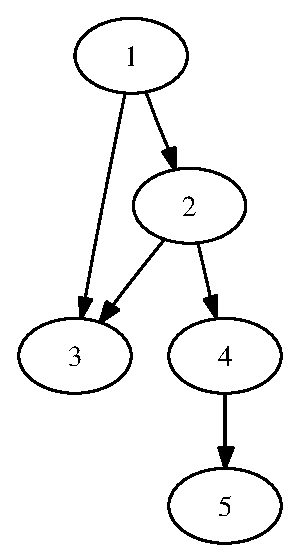
\epsfig{file=Figures/graph0,scale=0.6}

  \caption{A simple graph.}
  \label{fig:graph0}
\end{figure}



\noindent
The graph given by the relation \texttt{R} contains only the direct connections of vertices.  For example, in
the graph shown in Figure \ref{fig:graph0}, there is a direct connection from vertex $1$ to vertex $2$ and
another direct connection from vertex $2$ to vertex $4$.  Intuitively, vertex $4$ is reachable from vertex $1$,
since from vertex $1$ we can first reach vertex $2$ and from vertex $2$ we can then reach vertex $4$.  However,
there is is no direct connection between the vertices $1$ and $4$.  To make this more formal, define
a \blue{path} of a graph $R$ as a list of vertices
\\[0.2cm]
\hspace*{1.3cm}
$[x_1, x_2, \cdots, x_n]$ \quad such that \quad $\pair(x_i,x_{i+1}) \in R$ \quad for all $i=1,\cdots,n-1$.
\\[0.2cm]
In this case, the path $[x_1, x_2, \cdots, x_n]$ is written as
\\[0.2cm]
\hspace*{1.3cm}
$x_1 \mapsto x_2 \mapsto \cdots \mapsto x_n$
\\[0.2cm]
and has the \blue{length} $n-1$, since there are $n-1$ direct connections of the form $\pair(x_i,x_{i+1})$ that
make up this path.
To put it differently,  the length of a path
$[x_1,x_2,\cdots,x_n]$ is defined as the number of edges connecting the vertices and not as the
number of vertices appearing on the path.

Furthermore,  two vertices $a$ and $b$ of a graph are said to be \blue{connected} \index{connected} iff there exists a path
\\[0.2cm]
\hspace*{1.3cm}
$[x_1,\cdots,x_n]$ \quad such that \quad $a = x_1$ \quad and \quad $b = x_n$.
\\[0.2cm]
The goal of this section is to develop an algorithm that checks whether two vertices $a$ and $b$ are connected.
Furthermore, we want to be able to compute the corresponding path connecting the vertices $a$ and $b$.

\subsection{Breadth-First Search}
We are now ready to present \blue{breadth-first search} \index{breadth-first search}.  This is an algorithm
for finding a path in a given graph.  Figure \ref{fig:Breadth-First-Search.ipynb} on page
\pageref{fig:Breadth-First-Search.ipynb} shows the function \texttt{search}.  This function uses three
arguments:
\begin{enumerate}[(a)]
\item $R$ is a binary relation that is interpreted as a directed graph.
\item \texttt{start} and \texttt{goal} are nodes in this graph.
\end{enumerate}
The function search returns a path leading from \texttt{start} to  \texttt{goal} if such a path exists.
Otherwise it returns \texttt{None}.  We discuss the implementation of the function \texttt{search} line by line.

\begin{figure}[!ht]
  \centering
\begin{minted}[ frame         = lines, 
                framesep      = 0.3cm, 
                numbers       = left,
                numbersep     = -0.2cm,
                bgcolor       = sepia,
                xleftmargin   = 0.8cm,
                xrightmargin  = 0.8cm,
              ]{python3}
    def search(R, start, goal):
        Paths   = { (start,) }
        Visited = { start }
        while True:
            NewPaths = set()
            for Path in Paths:
                for (y, z) in R:
                    if Path[-1] == y and z not in Visited:
                        LongerPath = Path + (z,)
                        if z == goal:
                            return LongerPath
                        NewPaths.add(LongerPath)
                        Visited .add(z)
            if NewPaths == set():
                return
            Paths = NewPaths
\end{minted} 
\vspace*{-0.3cm}
\caption{Breadth-first search.}  \label{fig:Breadth-First-Search.ipynb}
\end{figure} %\$


\begin{enumerate}
\item In line 2 we initialize the variable \texttt{Paths} to contain the path that starts in the node
      \texttt{start} and has the length $0$.  After the $n$th iteration of the \texttt{while} loop in line 4,
      the set \texttt{Paths} will contain all paths in the graph that start in node \texttt{start} and have a
      length of $n$.
\item In line 3 we initialize the set \texttt{Visited} to contain the state \texttt{start}.
      Every time we discover a new node, it is added to the set \texttt{Visited}.
      The reason is that we want all the paths stored in the set \texttt{Paths} to be shortest paths.
      Therefore, we only add a new path to this set if the end point of this path has not yet been visited.
\item Before the $n$th iteration of the \texttt{while} loop in line 4 all paths stored in
      the set \texttt{Paths} have a length of $n-1$.  The purpose of the next iteration is to extend the paths to
      a length of $n$.  Those paths that can not be extended are discarded.     
\item \texttt{NewPaths} is the set of those paths that have been extended.  In the $n$th iteration,
      all paths in this set will have a length of $n$.
\item In line 6 to 8 we iterate over all paths discovered so far that end in the node $y$, where $\langle y, z\rangle$
      is a pair in the relation $R$ and the node $z$ has not yet been visited.
\item If we find such a path \texttt{Path} we extend it by appending the node $z$.
\item If $z$ is equal to \texttt{goal} we have found a path from \texttt{start} to \texttt{goal} and return
      this path.
\item Otherwise, this new path is added to the set \texttt{NewPaths} and the node $z$ is added to the set
      \texttt{Visited} to record the fact that we now have found a path leading to $z$.
\item If we do not find any new path in a given iteration, then there is no path from \texttt{start} to
      \texttt{goal} and the function returns.
\item Otherwise, \texttt{Paths} is set to \texttt{NewPaths} and the loop repeats.
\end{enumerate}


\subsection{The Wolf, the Goat, and the Cabbage}
\index{wolf, goat, and cabbage}
Next, we present an application of the theory developed so far.  We solve a problem that has puzzled
the greatest agricultural economists for centuries.  The puzzle we want to solve is known as the 
\href{http://jeux.lulu.pagesperso-orange.fr/html/anglais/loupChe/loupChe1.htm}{wolf-goat-cabbage puzzle}:  
\vspace*{0.3cm}

\begin{minipage}[c]{16cm}
{\sl
An agricultural economist has to sell a wolf, a goat, and a cabbage on a market place.  In order to
reach the market place, she has to cross a river.  The boat that she can use is so small that it can
only accommodate either the goat, the wolf, or the cabbage in addition to the agricultural economist.
Now if the agricultural economist leaves the wolf alone with the goat, the wolf will eat the goat.
If, instead, the agricultural economist leaves the goat with the cabbage, the goat will eat the cabbage.
Is it possible for the agricultural economist to develop a schedule that allows her to cross the river
without either the goat or the cabbage being eaten?
}
\end{minipage}
\vspace*{0.3cm}

\noindent
In order to compute a schedule, we first have to model the problem.  The various \blue{states} of the problem will
be regarded as \blue{vertices} of a graph and this graph will be represented as a binary relation.
To this end we define the set
\begin{verbatim}
  All = {'farmer', 'wolf, 'goat', 'cabbage'}.
\end{verbatim}
Every node will be represented as a subset \texttt{S} of the set \texttt{All}.  The idea is that the set \texttt{S}
specifies those objects that are on the left side of the river.  We assume that initially the farmer and his goods
are on the left side of the river. 
Therefore, the set of all states that are \blue{allowed} according to the specification of the problem can be defined
as the set 
\begin{verbatim}
  States = { S for S in power(All) if not problem(S) and not problem(All-S) }
\end{verbatim}
Here, we have used the procedure \texttt{problem} to check whether a given set \texttt{S} has a problem,
where a problem is any situation where either the goat eats the cabbage or the wolf eats the goat.
Note that since \texttt{S} is the set of objects on the left side, the expression $\texttt{All-S}$
computes the set of objects on the right side of the river.

Formally, a set \texttt{S} of objects has a problem if both of the following conditions
are satisfied:
\begin{enumerate}
\item The farmer is not an element of \texttt{S} and
\item either \texttt{S} contains both the goat and the cabbage or \texttt{S} contains both the wolf and the goat.
\end{enumerate}
Therefore, we can implement the function \texttt{problem} as follows:
\begin{verbatim}
  def problem(S):
      return ('farmer' not in S) and             \
             (('goat' in S and 'cabbage' in S) or   # goat eats cabbage
              ('wolf' in S and 'goat'    in S)   )  # wolf eats goat
\end{verbatim}
Note that we have to use a \blue{line continuation backslash} ``\texttt{$\backslash$}''
at the end of the first line of the return statement.
We do not need a continuation backslash at the end of the second line of the return statement since
the opening parenthesis at the beginning of the second line has not yet been closed when the second line
finishes and therefore \textsl{Python} is able to figure out that the expression defined in this line is
continued in the third line.

We proceed to compute the relation \texttt{R} that contains all possible transitions between
different states.  We will compute \texttt{R} using the formula:
\\[0.2cm]
\hspace*{0.75cm}
\texttt{R = R1 + R2;}
\\[0.2cm]
Here \texttt{R1} describes the transitions that result from the farmer crossing the river from left
to right, while \texttt{R2} describes the transitions that result from the farmer crossing the river
from right to left.  We can define the relation \texttt{R1} as follows:
\begin{verbatim}
  R1 = { (S, S-B) for S in States 
                  for B in power(S)
                  if S-B in States and 'farmer' in B and len(B) <= 2
       }
\end{verbatim}
Let us explain this definition in detail:
\begin{enumerate}
\item Initially, \texttt{S} is the set of objects on the left side of the river.  Hence, \texttt{S}
      is an element of the set of all states that we have defined as \texttt{States}.
\item \texttt{B} is the set of objects that are put into the boat and that do cross the river.  Of
      course, for an object to go into the boat is has to be on the left side of the river to begin
      with.  Therefore, \texttt{B} is a subset of \texttt{S} and hence \texttt{B} is an element of the power set
      of \texttt{S}. 
\item Therefore  \texttt{S-B} is the set of objects that are left on the left side of the river after
      the boat has crossed.  Of course, the new state \texttt{S-B} has to be a state that does not
      have a problem.  Therefore, we check that the set \texttt{S-B} is an element of the set \texttt{States}.
\item Furthermore, the farmer has to be inside the boat.  This explains the condition 
      \\[0.2cm]
      \hspace*{1.3cm}
      \texttt{\symbol{39}farmer\symbol{39} in B}.
\item Finally, the boat can only have two passengers.  Therefore, we have added the condition
      \\[0.2cm]
      \hspace*{1.3cm}
      \texttt{len(B) <= 2}.
\end{enumerate}
Next, we have to define the relation \texttt{R2}.  However, as crossing the river from right to left
is just the reverse of crossing the river from left to right, \texttt{R2} is just the \blue{inverse} of
\texttt{R1}.   Hence we define:
\begin{verbatim}
  R2 = { (S2, S1) for (S1, S2) in R1 }.
\end{verbatim}
Next, the relation \texttt{R} is the union of \texttt{R1} and \texttt{R2}:
\begin{verbatim}
  R = R1 | R2.
\end{verbatim}
Finally, the start state has all objects on the left side.  Therefore, we have
\begin{verbatim}
  start = All.
\end{verbatim}
In the end, all objects have to be on the right side of the river.  That means that nothing is left
on the left side.  Therefore, we define
\begin{verbatim}
  goal = {}.
\end{verbatim}


\begin{figure}[h]
  \centering

  \epsfig{file=Figures/wolf-goat-cabbage, scale=0.4}

  \caption{The relation \texttt{R} shown as a directed graph.}
  \label{fig:wolf-goat-cabbage.pdf}
\end{figure}



\noindent
Figure \ref{fig:wolf-goat-cabbage.pdf} on page \pageref{fig:wolf-goat-cabbage.pdf} displays the relation $R$ graphically.
Figure \ref{fig:wolf-ziege} on page \pageref{fig:wolf-ziege} shows the program
\href{https://github.com/karlstroetmann/Logic/blob/master/Python/wolf-goat-cabbage.py}{\texttt{wolf-goat-cabbage.py}}
that combines the statements shown so far.  The solution computed by this program is shown in Figure
 \ref{fig:wolf-ziege-solution}.

\begin{figure}[!ht]
  \centering
\begin{minted}[ frame         = lines, 
                framesep      = 0.3cm, 
                numbers       = left,
                numbersep     = -0.2cm,
                bgcolor       = sepia,
                xleftmargin   = 0.3cm,
                xrightmargin  = 0.3cm,
              ]{python3}
    def problem(S):
        return ('farmer' not in S) and             \
               (('goat' in S and 'cabbage' in S) or   # goat eats cabbage
                ('wolf' in S and 'goat'    in S)   )  # wolf eats goat
    
    All   = frozenset({ 'farmer', 'wolf', 'goat', 'cabbage' })
    R1    = { (S, S - B) for S in States for B in power(S)
                         if S - B in States and 'farmer' in B and len(B) <= 2
            }
    R2    = { (S2, S1) for (S1, S2) in R1 }
    R     = R1 | R2
    start = All
    goal  = frozenset()
    Path  = findPath(start, goal, R)
\end{minted} 
\vspace*{-0.3cm}
\caption{Solving the wolf-goat-cabbage problem.}  
\label{fig:wolf-ziege}
\end{figure}


\begin{figure}[!ht]
  \centering
\begin{minted}[ frame         = lines, 
                framesep      = 0.3cm, 
                numbers       = left,
                numbersep     = -0.2cm,
                bgcolor       = sepia,
                xleftmargin   = 0.8cm,
                xrightmargin  = 0.8cm,
              ]{python3}
    {'cabbage', 'farmer', 'goat', 'wolf'}                                 {}
                             >>>> {'farmer', 'goat'} >>>> 
    {'cabbage', 'wolf'}                                   {'farmer', 'goat'}
                             <<<< {'farmer'} <<<< 
    {'cabbage', 'farmer', 'wolf'}                                   {'goat'}
                             >>>> {'farmer', 'wolf'} >>>> 
    {'cabbage'}                                   {'farmer', 'goat', 'wolf'}
                             <<<< {'farmer', 'goat'} <<<< 
    {'cabbage', 'farmer', 'goat'}                                   {'wolf'}
                             >>>> {'cabbage', 'farmer'} >>>> 
    {'goat'}                                   {'cabbage', 'farmer', 'wolf'}
                             <<<< {'farmer'} <<<< 
    {'farmer', 'goat'}                                   {'cabbage', 'wolf'}
                             >>>> {'farmer', 'goat'} >>>> 
    {}                                 {'cabbage', 'farmer', 'goat', 'wolf'}
\end{minted} 
\vspace*{-0.3cm}
\caption{A schedule for the agricultural economist.}  
\label{fig:wolf-ziege-solution}
\end{figure}
\pagebreak
\vspace*{\fill}



\section{Symbolic Differentiation}
\index{symbolic differentiation}
In this section we will develop a program that reads an arithmetic expression like the string
\\[0.2cm]
\hspace*{1.3cm}
\texttt{\symbol{34}x * exp(x)\symbol{34}},
\\[0.2cm]
interprets this string as describing the real valued function 
\\[0.2cm]
\hspace*{1.3cm}
$x \mapsto x \cdot \exp(x)$, 
\\[0.2cm]
and then takes the derivative of this function with respect to the variable $x$.  In order to specify the input
of this program more clearly, we first define the notion of an \blue{arithmetic expression} inductively.
\begin{enumerate}[(a)]
\item Every number $c \in \mathbb{R}$ is an arithmetic expression.
\item Every variable $v$ is an arithmetic expression.
\item If $s$ and $t$ are arithmetic expressions, then
      \\[0.2cm]
      \hspace*{1.3cm}
      $s + t$, \quad $s - t$, \quad $s * t$, \quad $s / t$, \quad and \quad $s \,\mathtt{**}\, t$
      \\[0.2cm]
      are arithmetic expressions.  Here $s \,\mathtt{**}\, t$ is interpreted as $s^t$.
      
\item If $e$ is an arithmetic expression, then both
      \\[0.2cm]
      \hspace*{1.3cm}
      $\exp(e)$ \quad and \quad $\ln(e)$
      \\[0.2cm]
      are arithmetic expressions.
\end{enumerate}
We want do implement a function \texttt{diff} that takes two arguments:
\begin{enumerate}
\item The first argument \texttt{expr} is an arithmetic expression.
\item The second argument \texttt{var} is the name of a variable.
\end{enumerate}
The function call \texttt{diff(expr, var)} will then compute the derivative of \texttt{expr} with respect to the variable \texttt{var}.  For example, the function call \texttt{diff(\symbol{34}x*exp(x)\symbol{34}, \symbol{34}x\symbol{34})} will compute the output
\\[0.2cm]
\hspace*{1.3cm}
\symbol{34}\texttt{1*exp(x) + x*exp(x)}\symbol{34}
\\[0.2cm]
because we have:
$$ \frac{\mathrm{d}\;}{\mathrm{d}x} \bigl( x \cdot \mathrm{e}^x \bigr) = 1 \cdot x + x \cdot \mathrm{e}^x $$
It would be very tedious to \blue{represent} arithmetic expressions as strings.  Instead, we will represent
arithmetic expressions as \blue{nested tuples}.  \index{nested tuple}
The notion of a \emph{nested tuple} is defined inductively:
\begin{itemize}
\item $\langle x_1, x_2, \cdots, x_n \rangle$ is a nested tuple if each of the components $x_i$ is either a
      number, a string, or is itself a nested tuple.
\end{itemize}
For example, the arithmetic expression ``\texttt{x*exp(x)}'' is represented as the nested tuple
\\[0.2cm]
\hspace*{1.3cm}
$\bigl\langle\texttt{\symbol{34}}*\texttt{\symbol{34}}, \texttt{\symbol{34}}x\texttt{\symbol{34}}, \langle \texttt{\symbol{34}}\mathtt{exp}\texttt{\symbol{34}}, \texttt{\symbol{34}}x\texttt{\symbol{34}} \rangle\bigr\rangle$.
\\[0.2cm]
In order to be able to convert string into nested tuples, we need a \blue{parser}.
\index{parser}
  A parser is a program that
takes a string as input and transforms this string into a nested tuple, which is then returned as a result.
I have implemented a parser in the file ``\texttt{exprParser.py}''.  The details of the implementation of this
parser will be discussed in the lecture on
\href{https://github.com/karlstroetmann/Algorithms/blob/master/Lecture-Notes/algorithms.pdf}{algorithms} in the
second semester..

\noindent
The function \texttt{diff} that is shown in Figure \ref{fig:diff.py} on page \pageref{fig:diff.py} is part
of the program
\href{https://github.com/karlstroetmann/Logic/blob/master/Python/Symbolic-Differentiation.ipynb}{\texttt{Symbolic-Differentiation.ipynb}}.
This function is called with one argument:
The argument \texttt{e} is an arithmetic expression.
The function \texttt{diff} interprets its argument \texttt{e} as a function of the variable
\texttt{x}.  We take the \href{https://en.wikipedia.org/wiki/Derivative}{derivative} of this
function with respect to the variable \texttt{x}.  For example, in order to compute the derivative of
the function
\\[0.2cm]
\hspace*{1.3cm}
$x \mapsto x^x$,
\\[0.2cm]
we can call the function  \texttt{diff} as follows:
\\[0.2cm]
\hspace*{1.3cm}
\texttt{diff(\symbol{34}x ** x\symbol{34})}.
\\[0.2cm]
Let us now discuss the implementation of the function \texttt{diff} in more detail.  
\begin{enumerate}
\item The lines 3 - 6 implement the rule: 
      $$\frac{\mathrm{d}\;}{\mathrm{d}x}\bigl(f(x) + g(x)\bigr) = \frac{\mathrm{d}\;}{\mathrm{d}x} f(x) + \frac{\mathrm{d}\;}{\mathrm{d}x} g(x)$$
\item Line 7 - 10 implement the rule:
      $$\frac{\mathrm{d}\;}{\mathrm{d}x}\bigl(f(x) - g(x)\bigr) = \frac{\mathrm{d}\;}{\mathrm{d}x} f(x) - \frac{\mathrm{d}\;}{\mathrm{d}x} g(x)$$      
\item Line 11 - 14 deals with the case where \texttt{e} is a product.  The 
      \href{https://en.wikipedia.org/wiki/Product\_rule}{product rule} is      
      $$ \frac{\mathrm{d}\;}{\mathrm{d}x}\bigl(f(x) \cdot g(x)\bigr) = \left(\frac{\mathrm{d}\;}{\mathrm{d}x} f(x)\right)\cdot g(x) + f(x) \cdot \left(\frac{\mathrm{d}\;}{\mathrm{d}x} g(x)\right)
      $$
\item Line 15 - 17 deals with the case where \texttt{e} is a quotient.  The
      \href{https://en.wikipedia.org/wiki/Quotient\_rule}{quotient rule} is
      $$ \frac{\mathrm{d}\;}{\mathrm{d}x}\left(\frac{f(x)}{g(x)}\right) = 
         \frac{\displaystyle\left(\frac{\mathrm{d}\;}{\mathrm{d}x} f(x)\right)\cdot g(x) - 
         f(x) \cdot \left(\frac{\mathrm{d}\;}{\mathrm{d}x} g(x)\right)}{g(x) \cdot g(x)}
      $$      
\item Line 19 - 21 deals with the case where \texttt{e} is a power.  Now in order to take the derivative of an
      expression of the form
      $$  f(x)^{g(x)} $$
      we first need to rewrite this expression using the following trick:
      $$ f(x)^{g(x)} = \exp\bigl(\ln\bigl(f(x)^{g(x)}\bigr)\bigr) = \exp\bigl(g(x) \cdot \ln(f(x))\bigr) $$
      Then, we can recursively call \texttt{diff} for this expression.  This works, because the function
      \texttt{diff} can deal with both the exponential function $x \mapsto \exp(x)$ and with the natural
      logarithm $x \mapsto \ln(x)$.  This rewriting is done in line 21.      
\item Line 22-25 deals with the case where \texttt{e} has the form 
      $$\ln\bigl(f(x)\bigr)$$  
      In order to take the derivative of this expression, we first need to know the derivative of the natural
      logarithm.  This derivative is given as     
      $$ \frac{\mathrm{d}\;}{\mathrm{d}x} \ln(x) = \frac{1}{x}$$
      Then, using the \href{https://en.wikipedia.org/wiki/Chain\_rule}{chain rule} we have that
      $$ \frac{\mathrm{d}\;}{\mathrm{d}x} \ln\bigl(f(x)\bigr) = \frac{\frac{\mathrm{d}\;}{\mathrm{d}x} f(x)}{f(x)}$$     
\item Line 26 - 29 deals with the case where \texttt{e} has the form $\exp\bigl(f(x)\bigr)$.  
      In order to take the derivative of this expression, we first need to know the derivative of the 
      \href{https://en.wikipedia.org/wiki/Exponential\_function}{exponential function}.  
      This derivative is given as 
      $$ \frac{\mathrm{d}\;}{\mathrm{d}x} \exp(x) = \exp(x)$$    
      Then, using the \href{https://en.wikipedia.org/wiki/Chain\_rule}{chain rule} we have that
      $$\frac{\mathrm{d}\;}{\mathrm{d}x} \exp\bigl(f(x)\bigr) = \left(\frac{\mathrm{d}\;}{\mathrm{d}x} f(x)\right) \cdot \exp\bigl(f(x)\bigr) $$
\item Line 30-31 deals with the case where \texttt{e} is a variable and happens to be the same variable as
      \texttt{x}.  This is checked using the condition    
      \texttt{e == x}.  As we have
      $$\frac{\mathrm{d}x}{\mathrm{d}x} = 1,$$
      the function \texttt{diff} returns \texttt{1} in this case.  
\item Otherwise, the expression is assumed to be a constant and hence we return 0.
\end{enumerate}


\begin{figure}[!ht]
\centering
\begin{minted}[ frame         = lines, 
                framesep      = 0.3cm, 
                firstnumber   = 1,
                numbers       = left,
                numbersep     = -0.2cm,
                bgcolor       = sepia,
                xleftmargin   = 0.8cm,
                xrightmargin  = 0.8cm,
              ]{python3}
    def diff(e):
        'differentiate the expressions e with respect to the variable x'
        if e[0] == '+':
            f , g  = e[1:]
            fs, gs = diff(f), diff(g)
            return ('+', fs, gs)
        if e[0] == '-':
            f , g  = e[1:]
            fs, gs = diff(f), diff(g)
            return ('-', fs, gs)
        if e[0] == '*':
            f , g  = e[1:]
            fs, gs = diff(f), diff(g)
            return ('+', ('*', fs, g), ('*', f, gs))
        if e[0] == '/':
            f , g  = e[1:]
            fs, gs = diff(f), diff(g)
            return ('/', ('-', ('*', fs, g), ('*', f, gs)), ('*', g, g))
        if e[0] == '**':
            f , g  = e[1:]
            return diff(('exp', ('*', g, ('ln', f))))
        if e[0] == 'ln':
            f  = e[1]
            fs = diff(f) 
            return ('/', fs, f)
        if e[0] == 'exp':
            f  = e[1]
            fs = diff(f) 
            return ('*', fs, e)
        if e == 'x':
            return '1'
        return 0                  
\end{minted}
\vspace*{-0.3cm}
\caption{A function for symbolic differentiation}
\label{fig:diff.py}
\end{figure}


In order to test this function we can implement a function \texttt{test} as shown in Figure \ref{fig:test-diff.py}.
Then the expression
\\[0.2cm]
\hspace*{1.3cm}
\texttt{diff(\symbol{34}x ** x\symbol{34})}
\\[0.2cm]
yields the result:
\\[0.2cm]
\hspace*{1.3cm}
d/dx x ** x = (1*ln(x) + x*1/x)*exp(x*ln(x))
\\[0.2cm]
This shows that
\\[0.2cm]
\hspace*{1.3cm}
$\ds \frac{\mathrm{d}\;}{\mathrm{d}x} x^x = \bigl(\ln(x) + 1\bigr) \cdot \exp\bigl(x \cdot \ln(x)\bigr) =
 \bigl(\ln(x) + 1\bigr) \cdot x^x
$.


\begin{figure}[!ht]
\centering
\begin{minted}[ frame         = lines, 
                framesep      = 0.3cm, 
                firstnumber   = 1,
                numbers       = left,
                numbersep     = -0.2cm,
                bgcolor       = sepia,
                xleftmargin   = 0.8cm,
                xrightmargin  = 0.8cm,
              ]{python3}
    import exprParser as ep

    def test(s):
        t = ep.ExprParser(s).parse()
        d = diff(t)
        print(f'd/dx {s} = {ep.toString(d)}')
\end{minted}
\vspace*{-0.3cm}
\caption{Testing symbolic differentiation.}
\label{fig:test-diff.py}
\end{figure}





%%% Local Variables:
%%% mode: latex
%%% TeX-master: "logic"
%%% End:
